%!TEX root = ../masters_thesis.tex

\section{Uncertainty} % (fold)
\label{sec:uncertainty}

Every aspect of the concept (section \ref{sec:concept}) and the development (section \ref{sec:development}) of this work is based on the prerequisite of full certainty of the data. That means both the Historical-Geographic Operations and the Hivent-Based Spatio-Temporal Data Model assume that the dates of the historical events, the names and territories of the historical and current areas and the historical relations between events and areas are correct, accurate, exact and precise (definitions see \ref{sub:types_of_uncertainty}).

However, this assumption is far from valid. In historical research, uncertainty is one of the major problems (see \ref{ssub:history}) a historian has to deal with on a daily basis: sources, even primary sources, can be biased towards the author of the source, information can be imprecise or inaccurate and information can be conflicting with other sources. The purpose of this section is to introduce the problem of uncertainty in the domain of this thesis, explain the main concepts and develop solutions to deal with this problem.


% ==============================================================================
\subsection{Definition of a Country} % (fold)
\label{sub:definition_of_a_country}

The problem begins with the definition of a term that almost everybody in the world is familiar with: a ``country''. But the search for a non-conflicting explanation of what a country actually is leads to a dead end.

The Oxford Dictionary definition of a country reads as follows:
\begin{quote}
  ``The \emph{territory} of a \emph{nation}; a \emph{region} constituting an \emph{independent state}, or a region, province, etc., which was once independent and is still distinct in institutions, language, etc.''
  \footnote{\textit{country, n. and adj}, Oxford English Dictionary, URL: \url{http://www.oed.com/view/Entry/43085?}, last access: 2016-04-25}
\end{quote}

This definition includes many different concepts and terms: the territory or region that the country is on, a nation or state, and a cultural population of the territory in terms of institutions or languages. While nation and state are commonly used as synanyms for countries, their meaning varies from case to case, as it will be examined in this section.

The CIA Factbook collects, manages and visualizes data and facts ``on every country, dependency, and geographic entity in the world''. Its definition of a country should therefore be helpful to understand what a country actually is. In the database the term \emph{political entity} is defined like this:
\begin{quote}
  An ``Independent state refers to a people politically organized into a sovereign state with a \emph{definite territory}. \emph{Dependencies} and \emph{areas of special sovereignty} refer to a broad category of political entities that are associated in some way with an independent state.''
  \footnote{\textit{The World Factbook}, CIA Factbook, URL: \url{https://www.cia.gov/library/publications/the-world-factbook/docs/notesanddefs.html\#T}, last access: 2016-04-25}
\end{quote}

The CIA Factbook includes a total of 267 ``separate geographic entities'':
\begin{enumerate}
  \item 195 independent states (e.g. Germany, the United Kingdom or Swaziland)
  \item 2 ``other'' states (Taiwan and the European Union),
  \item 85 ``dependencies and areas of special sovereignty'' (e.g. Greenland to Denmark, Hong Kong to China or Puerto Rico to the United States),
  \item 6 ``miscellaneous'' entities (Antarctica, the Gaza Strip, Paracel Islands, Spratly Islands, West Bank, Western Sahara) and
  \item 5 ``other entitites'' (the Arctic, Atlantic, Indian, Pacific and Southern Ocean)
\end{enumerate}

Excluding ``other entities'', there are four different groups of political entities used in the Factbook. While Antarctica as an uninhabitated place might not be a surprising miscellaneous entity, the Gaza Strip and the West Bank as the two territories associated to Palestine, Taiwan, Hong Kong or Greenland are not listed as independent states, although they practically do to a large degree.

The United Nations as an intergovernmental organisation is probably the most important source for countries around the world. It was found after World War II (October 1945) and promotes international peace keeping, security, protection of human rights or humanitarian aid. The committee has 193 full member states and two permanent obervers: The Holy See (Vatican City) and the State of Palestine. \cite{UNmembers}

% ------------------------------------------------------------------------------
\subsubsection{Special Cases} % (fold)
\label{ssub:special_cases}

Examining the list of the CIA Factbook and the UN member states yield several interesting observations and special cases, which can be classified by their degree of recognition and their membership status in the United Nations.


\paragraph{UN observer states} % (fold)
\label{par:un_observer_states}

The \emph{Holy See} is the juridcal and spiritual entity representing the territory of Vatican City. It is classified as an independent state by the CIA but is not a full member of the UN, because it has never applied for it. However, it is a fully sovereign country with diplomatic relations to the vast majority of countries in the world -- which makes it the by far smallest sovereign state in the world (0.44 m²), inside the city of Rome with a population of only 800 people, including 30 women \cite{VaticanPopulation}.

The \emph{State of Palestine} consists of the territories of the West Bank, East Jerusalem and the Gaza Strip and has a population of 4.8 million people \cite[as of 2016]{PalestinePopulation}. While it is also an observer state it is in a totally different situation in terms of sovereignty: First of all, it does not have a clearly defined territory, because the borders of Palestine drawn in the 1949 Green Line Armistice Agreement were never intended to be used as international boundaries \cite{PalestineTerritory}. Since then, the ongoing and complex conflict with the State of Israel lead to a difficult situations regarding the sovereignty over the territories of Palestine. Additionally, while 114 states officially recognize the Palestinian state, almost all current main economic powers do not, including the Canada, France, Germany, Italy, the United Kingdom and the United States. None of them even voted in favor of Palestine receiving an observing status in the UN \cite{PalestineUN}. That means, unlike the Holy See, Palestine is not a fully sovereign and recognized state.

% paragraph un_observer_states (end)

\paragraph{UN non-members with limited recognition} % (fold)
\label{par:un_non_members_with_limited_recognition}

\emph{Kosovo} is listed by the CIA Factbook as an independend nation, after having seceded from Serbia and declared independence in 2008. It has a clearly defined territory and population and is recognized by 111 UN member states. However, among the five permanent members of the United Nations Security Council (USA, UK, France, Russia and China), the latter two veto the membership of Kosovo in the United Nations -- but UN membership requires full approval by all members of the security council. Therefore, Kosovo is not even an observer state of the United Nations, although having about the same degree of international recognition as Palestine \cite{KosovoThanksYou}.

The status of Taiwan is a very complicated issue. An overgeneralized description of the problem, which involves two territories and two political entities, is: There is the \emph{People's Republic as China} (commonly known as China) with full control over mainland China and the \emph{Republic of China}, governing the island of Taiwan. However, both political entities claim each others land. That means, there are two states claiming the exact same territory. But, since 1971 the People's Republic of China is the representative of whole China in the United Nations, including the island of Taiwan. Because it is part of the Security Council, it successfully vetos membership requests of Taiwan. Therefore, the Republic of China can not be a member of the United Nations, although it operates like an independend country by international standards: They have an own jurisdiction, issue own passports and have unofficial diplomatic relations to most countries in the world. But officially, only 22 member states of the United Nations uphold diplomatic relations to Taiwan \cite{TaiwanRecognition}. To all of these states the Republic of China does not have any diplomatic relations, which makes it an only partially recognized state.

There are other non-member states of the United Nations which have not yet gained broad international recognition: the Sahrawi Arab Democratic Republic (recognized by 84 UN member states \cite{WesternSaharaRecognition}), Abkhazia (6 \cite{AbkhaziaRecognition}), South Ossetia (5 \cite{SouthOssetiaRecognition}), the Turkish Republic of Northern Cyprus (1 \cite{NorthernCyprusRecognition}) Nagorno-Karabakh Republic (0 \cite{NagornoRecognition}), Transnistria (0 \cite{TransnistriaRecognition}) and Somaliland (0 \cite{SomalilandRecognition}).

% paragraph un_non_members_with_limited_recognition (end)

\paragraph{UN members with limited recognition} % (fold)
\label{par:un_members_with_limited_recognition}

In Addition to the Republic of China, there are five other member states of the United Nations that are not fully recognized by all other UN members: Armenia (not recognized by Pakistan \cite{ArmeniaRecognition}), the Republic of Cyprus (not recognized by Turkey \cite{CyprusRecognition}), North and South Korea (officially Democratic People's Republic of Korea and Republic of Korea, mutual non-recognition \cite{KoreaRecognition}) and the State of Israel, which 32 UN member states do not recognize \cite{IsraelRecognition}.

% paragraph un_members_with_limited_recognition (end)

\paragraph{Special Territories} % (fold)
\label{par:special_territories}

Additionally to countries gaining for international recognition there are territories belonging to fully sovereign countries with a varying degree of sovereignty. For example Greenland is an autonomous country within the Kingdom of Denmark, but not a member of the United Nations and therefore no sovereign state. The same applies to the Faroer Islands (part of Denmark) and numerous overseas territories of the United Kingdom, the French Republic and the Kingdom of the Netherlands in the Carribean, the Indian Ocean or the Southern Pacific Ocean. There are five countries in a so called \emph{Free Association}: Niue and Cook Islands to New Zealand and the Marshall Islands, the Federated States of Micronesia and Palau to United States. While New Zealands associations are quasi-independent nations, they are not part of the United Nations -- but the associations of the United States are full members of the UN \cite{SpecialTerritories}.

% TODO?
% example United Kingdom:  country?
% difference clear: geography             politics
%                   British Isles         United Kingdom of Great Britain and NI
%                     Great Britain         Scotland, England, Wales, Northern Ireland (province)
%                     Ireland             Republic of Ireland
%                     Shetland Islands
%                     Isle of Men
%                     ...

% Scotland, England and Wales are countries, but not sovereign states, Northern Ireland is a province and not a country. The UK is a constituent country, just like the Kingdom of the Netherlands and the Kingdom of Denmark.

% paragraph special_territories (end)

This incomplete and simplified list of special cases manifests the big problem that is associated with the terms ``country'', ``state'' or ``nations'': There is neither a \emph{de jure} consistent definition nor a \emph{de facto} consistent usage of these terms. Everything breaks down to two different concepts if statehood: The \emph{declaratory theory} and the \emph{constituitive theory}:


% subsubsection special_cases (end)

% ------------------------------------------------------------------------------
\subsubsection{Declaratory vs. Constituitive Theory} % (fold)
\label{ssub:declaratory_vs_constituitive_theory}

The declaratory theory, manifested in the Montevideo Convention 1933 \cite{MontevideoConvention}, gives each entity the right to declare a state if it matches all of the four requirements:
\begin{enumerate}
  \item a clearly defined territory
  \item a permanent population
  \item a political representation / government
  \item the \emph{capacity} to enter diplomatic relations
\end{enumerate}

These four requirements make sure that a state can exist physically and politically. However, it is worth noticing that this definition does not include any actual diplomatic relations to other states, but only the capacity. So the existance of a state is independent from its recognition by other states.

In contrast, the constituitive theory requires exactly that: A state can only be considered as such if it is recognized by other states. However, it is not defined anywhere by how many other states \cite{StateTheory}.

\begin{figure}[ht]
  \centering
  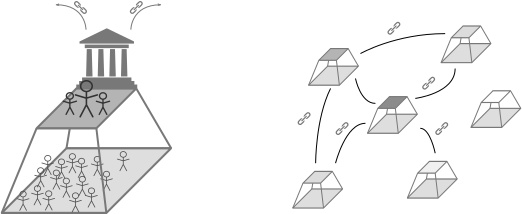
\includegraphics[width = 0.8\textwidth]{graphics/5-uncertainty/decl_const_theory}
  \caption{The Declaratory Theory (left) and the Constituitive Theory (right) of Statehood}
  \label{fig:declaratory_constituitive_theory}
\end{figure}

In summary, both theories can be explained as:
\begin{quote}
  ``A country is a country when it thinks it is a country''
  and \\
  ``A country is a country when other countries think that country is a country''
  \cite{greyCountries}
\end{quote}

Both theories have advantages and disadvantages, but the two main problems are:
\begin{enumerate}
  \item Following the declarative theory, countries are self-classifying and potentially conflicting entities. The application of this measure would grant Kosovo, the People's Republic of China, Abkhazia or the Sarhawi Arab Democratic Republic full statehood. However, since their territories are contested, this would lead to overlapping state territories which is impossible.
  \item There is no superior organization that can judge if a a country is a country or not. Even the United Nations fail to do so, because their membership requirements prevent states like Kosovo or the Republic of China from becoming full members. They have no power to rule out problems regarding the independence of Transnistria or Somaliland.
\end{enumerate}

Therefore it is impossible to objectivly classify an area as a country or not: nobody can say if the Republic of China, the State of Palestine or Niue are countries or not. On top of that, these theories have been introduced in the previous 80 years. For the time before 1933 the classification of a country is not just impossible, but also not justifyable because of a lack of jurisdiction.

That means, an historical geographic information system with the goal to visualize the development of the countries on Earth in time and space inevitably stores ``wrong'' information. Its data model can not fit self-classifying data and can not rely on an objective data source. The system has to contain approaches that deal with this problem.

% subsubsection declaratory_vs_constituitive_theory (end)

% subsection definition_of_a_country (end)


% ==============================================================================
\subsection{Types of Uncertainty} % (fold)
\label{sub:types_of_uncertainty}

In order to understand different types of uncertainty it is important to differentiate between \emph{precision} and \emph{accuracy}. When modelling a phenomenon on a real world, the more the model resembles the phenomenon, the more accurate or correct it is, i.e. the closer you get to the target, the higher the accuracy. Precision describes how close the results are away from each other, independent from the distance to the target. The smaller the variance of results, the higher the precision or exactness, i.e. if you get the same result over and over again, you are very precise. The goal for a data model is to be as accurate and precise as possible.

\begin{figure}[ht]
  \centering
  
\includegraphics[width = 0.35\textwidth]{graphics/5-uncertainty/accuracy_precision}
  \caption{The difference between accuracy and precision}
  \label{fig:accuracy_precision}
\end{figure}

Given the complexity and subjectivity in the domain of historical developments of countries, the data model in the concept of this thesis can be evaluated in terms of accuracy and precision.


\paragraph{Hivents} % (fold)
\label{par:evaluation_hivents}

model historically significant happenings with a focus on those who influence the geopolitical history of a country. The model contains only the following meta information: name, date and location of the event.

In modern history, geopolitical changes of countries are manifested mostly in historical treaties which are the result of a conference or any other gathering of representatives of stakeholders of that initiated change. Since each of those treaties is signed on one particular day, in one particular place and has one particular name, the ~\texttt{Hivent}~ model seems appropriate. However, it has several shortcomings in terms of precision:

The name of an historical event can have different versions: a long, official version and a short common version. The commonly known Treaty of Versailles (1919) is officially called the ``Treaty of Peace between the Allied and Associated Powers and Germany''. Also the name is different in other languages affected by the treaty. Additionally, there can be different versions of the name from different perspectives, even within the same language, e.g. XXX % TODO
The ~\texttt{Hivent}~ model does not account for different languages and versions and is therefore not very precise.

The ~\texttt{Hivent.date}~ is supposed to represent the temporal dimension of an historical event. While an historical change itself is discrete and happens at exactly one time point, the historical event yielding this change might not. The Congress of Vienna which reordered the empires on the European mainland was one of the main historical events in modern European history. While the changes of the congress came into effect on 9. June 1815, the congress itself took place in Vienna from September 1814 until June 1815 which is also a timespan of interest. Another phenomenon becomes apparent in the ``Convention for the Extension of Hong Kong Territory'' (1898) which had a predefined length of 99 years. The treaty therefore has two dates in which historical changes happened: the date the treaty came into effect and the date it stopped being in effect. Other interesting aspects are different calendar systems used in different parts of the world thoughout history: the October Revolution in Russia (1917) happened in November in their Gregorian Calendar system, but in October in the Julian Calendar. Also timezones can play a crucial role: The German Instrument of Surrender ending World War II in Europe came into effect on 8. May 1945 at 23:01 Central European, so the 8. May is celebrated as the Victory Day in Western Europe. But in the Soviet Union and nowadays Russia that happened at 1:01 Moscow Time on 9. May 1945 which is why the celebration of the Victory Day there happens one day later. While the ~\texttt{Hivent.date}~ field in the data model works with timezones, it does not support different calendar systems or multiple dates associated with one ~\texttt{Hivent}~ which limits its precision.

The event location is represented by the ~\texttt{Hivent.location}~ name of a place, which can e.g. be a city, a battlefield or a region. However, the first question arises regarding the relevance of the location: While the exact position of the battlefield of Verdun or the place where John F. Kennedy was assassinated might very relevant to the event itself, the location of a governmental bill, a declaration of independence or a border convention might not play an important role and usually happens in a representative place, e.g. the parliament or the office of a minister. In a lot of cases, it is much more important which territories an event actually influences instead of where it happened. The ~\texttt{Hivent}~ model is not very precise, because it does not support names in different languages, the actual geospatial location or region in which an historical event happened.

The even larger problem is an integral lack of accuracy: The whole nature of historical research is based on subjective interpretation of supposedly objective primary sources. But it is questionable if a source can actually be objective. Each bill, treaty or speech is written by somebody, each map was drawn by someone and has therefore a subjective note. Information in a primary source can be (un)intentionally incomplete, imprecise or inaccurate. The source can be biased towards the author, can contain secret passages not open to the public or its geographic information might be wrong. There are many problems involved in historical sources which makes the acquisition of objective historical data almost impossible. The further documents go back in time, the lower is the expected accuracy. Since all the information in the historical geographic information system is based on primary sources, the data in the system inherits these problems.

% paragraph evaluation_hivents (end)

\paragraph{Areas} % (fold)
\label{par:evaluation_areas}

model the main entity of the domain: historical or current countries. An ~\texttt{Area}~ represents one identical country, consisting at each time point of its existance of exactly one ~\texttt{AreaName}~ and one ~\texttt{AreaTerritory}. The model seems appropriate since the name and the territory of an area are exactly the two properties that are part of the domain. However, also those are problematic in terms of accuracy and precision.

The ~\texttt{Area}~ assumes a clear identification of each country. But as it has been discussed in subsection \ref{sub:definition_of_a_country} in detail, an objective decision of a country is impossible. Also, countries can be part of other autonomous (constituent) countries, like England is part of the United Kingdom of Great Britain and Northern Ireland or Greenland is part of Denmark. However, the data model does not support different levels of sovereignty, autonomy or international recognition.
% Additionally the historical context acquired by the start and end change that created or destroyed the ~\texttt{Area}~ can be ambiguous. While the motvation was to historically connect different countries to form an historical graph, the automatic deduction of historical succession from the historical geographic operations might not accurately replicate the identity of a state. An example is the German Democratic Republic which both historically and geographically seems to be a decendent of Allied-occupied Germany after World War II and therefore an indirect successor of the German Empire. However, the constitution of the GDR emphazised
% TODO: source? -> Berno
% think about it: is it really the case?

The ~\texttt{AreaName}~ has the same problem than the name of the ~\texttt{Hivent.name}: the name differs in other languages or can even differ between different cultures using the same language which the model does not support. But in one aspect it is more precise than for historical events, because it contains both the formal and the short name of a country.

More problematic is the ~\texttt{AreaTerritory}: Areas bordering international water have a constant coastline assuming that it has never changed. This is inaccurate, because coastlines gradually change all the time, therefore also the boundaries of the countries. The data model does support neither that nor international sea borders which are parts of a countries territory. The primary source for territories of countries are historical maps. They show the status of a country at one point in history or sometimes a territorial change. The process of extracting a boundary from an historical map is error-prone and yields to a loss of accuracy in each step on the way: digitizing, georeferencing and semi-automatic contour detection. Depending on the resolution, the map projection and the colors used in the map, these losses can range from minor to severe. In the data model it is not possible to provide information about the expected accuracy of a territory.

Another problem is that the territory is stored as a whole Polypolygon. Different parts of the border can have a different status, e.g. one part is a sea border, one is a well-established and demarcated border to neighboring country X and another part is a contested border to neighbour Y. The ~\texttt{AreaTerritory}~ data model does not account for these differences.

Lorem ipsum dolor sit amet, consectetur adipiscing elit. Nullam a ante urna. Ut lobortis eros et libero molestie lacinia. Maecenas ut placerat mi. Morbi eget fermentum turpis. Sed at lorem sit amet tellus tincidunt interdum at at diam. Vestibulum eros purus, ultrices aliquet ornare et, suscipit gravida massa. Sed eget dignissim neque.

Accurately modelling contested territories is also problematic. It is based on the principle that there can not be overlapping territories at the same time. That means, a contested territory, for example China or occupied territories in the State of Palestine by the State of Israel can only exist once at the same time and therefore have to treated specially. But the data model does not support contested areas. To go even further, it is questionnable which areas should be included in the data model and which not. While it seems obvious to have Spain, Saudi-Arabia and Azerbaijan in the system, the question of whether or not to include the State of Palestine, Abkhazia, Somaliland or micronations like the Conch Republic in the Florida Keys.

% paragraph evaluation_areas (end)

\paragraph{Uncertainty and Disagreement} % (fold)
\label{par:uncertainty_vs_disagreement}

are two different concepts that have to be differentiated at this point: if the border between the Principalities of Transsylvania and Wallachia is deducted from an historical map of 1600, the course of the border is uncertain (i.e. inaccurate) to a particular degree. On the other hand, the current border between India and Pakistan in the Kashmir region can be drawn with a high certainty (i.e. very precisely), but the parties disagree on the course of the border. Therefore, the Kashmir region is a contested territory. A data model that contains contested territories, would be accurately modelling the real world (a disagreement) and therefore be certain.


% paragraph uncertainty_vs_disagreement (end)


Overall, the current data model poorly accounts for different levels of uncertainty in historical geographic information: imprecise and inaccurate sources, different viewpoints and interpretations, contested territories, changing coastlines or different languages. The question of the upcoming subsection is: How can the data model be extended in order to be more accurate and more precise?


% subsection types_of_uncertainty (end)

% ==============================================================================
\subsection{Solution Approaches} % (fold)
\label{sub:solution_approaches}

The shortcomings of the current concept area:

\begin{enumerate}
  \item General
  \begin{enumerate}
    \item only one language (English)
    \label{problem_general_multilang}
    \item constant coastlines
    \label{problem_general_coastlines}
  \end{enumerate}
  \item Hivent
  \begin{enumerate}
    \item only one historical perspective on the Hivent name
    \label{problem_hivent_perspective}
    \item only one discrete Hivent date
    \label{problem_hivent_dates}
    \item only one calendar system (Julian Calendar)
    \label{problem_hivent_calendar}
    \item only location name, no connection to the map
    \label{problem_hivent_location}
  \end{enumerate}
  \item Area
  \begin{enumerate}
    \item only one historical perspective on the Area name
    \label{problem_area_perspective}
    \item all Areas on the same level (no dependencies)
    \label{problem_area_levels}
    \item no support for non-sovereign autonomous regions
    \label{problem_area_autonomy}
    \item no credibility of Areas existence (via international recognition)
    \label{problem_area_recognition}
    \item only clear territories, no support for neutral zones or contested territories
    \label{problem_area_territory}
    \item no support for uncertain parts of a territory
    \label{problem_area_territory_certainty}
    \item no support for international sea borders
    \label{problem_area_territory_sea_borders}
  \end{enumerate}
\end{enumerate}

A higher accuracy in the data model usually leads to a higher complexity. This trade-off has to be thoroughly be taken into consideration when supporting a new feature to make a model more accurate. This is why the following problems will be ignored in the rest of the section:
\begin{itemize}
  \item [\ref{problem_general_coastlines})] Coastlines change continually, therefore the Hivent-based spatio-temporal data model is not suitable to model their changes. A support for coastline changes would require another data model especially for coastlines, which is out of the scope of this thesis. One approach is to model international waters just like any other \texttt{Area} with an \texttt{AreaName} (name of the ocean) and an \texttt{AreaTerritory} and change the territories boundaries accordingto an underlying numerical solution over time. This way, the countries sharing that coastline as their international border would change likewise.
  \item[\ref{problem_hivent_perspective})] The support for different historical perspectives on the same event, e.g. different names and descriptions or even different historical changes would create a research tool with great potential. It would enable the possibility for different versions of history based on alternative scenarios (``What if X would have (not) happened?''). However, this would significantly increase the complexity of the system and would also be very subjective.
  \item[\ref{problem_hivent_calendar})] The introduction of different calendar systems would not increase the accuracy of the model significantly. The dates in the system must all stick to the Julian calendar, which is a reasonable requirement to avoid unnecessary complexity.
  \item[\ref{problem_area_perspective})] see \ref{problem_hivent_perspective})
  \item[\ref{problem_area_territory_sea_borders})] Currently each countries territory extends in a range of 3 to 12 miles (5 to 20 kilometers) \cite{UNSeaBorders} into international waters. While this is important to accurately model a territory, it is complex, because not every country has signed the convention and each signing party can choose their range into international water. This would not just increase the complexity of the model but also create unfamiliar country territories.
\end{itemize}

In order to tackle the remaining shortcomings of the current concept, both the user interface and the data model have to be extended.

% ------------------------------------------------------------------------------
\subsubsection{Extension of the Edit Mode} % (fold)
\label{ssub:extension_of_the_edit_mode}

The edit mode is extended by two new operations: (see figure \ref{fig:edit_mode_extension})
\begin{itemize}
  \item [\texttt{SCH}] change status of a country or territory
  \item [\texttt{REC}] declare new recognition (one country recognizes another one)
\end{itemize}

\begin{figure}[ht]
  \centering
  
\includegraphics[width = 0.6\textwidth]{graphics/5-uncertainty/edit_mode_extension.png}
  \caption{Newly designed and extended buttons for edit operations.}
  \label{fig:edit_mode_extension}
\end{figure}

Also the edit operation workflow gets changed. The first step (\texttt{SEL\_OLD\_AREA}) stays the same, but the second step (\texttt{SET\_NEW\_TERR}) that defines the territory of the new area(s) will be modified: Instead of drawing the whole territory as a set of polygons, the user draws one borderline at a time, geometrically as a polyline. This has the main advantage that each part of the border is treated separately.

The borderline is assigned a degree of certainty, in the interface controlled by a one-dimensional horizontal slider, in the model as a certainty value ~$\texttt{certainty} \in ]0 .. 1]$. Absolute certainty ($1.0$) creates a sharp and crisp line on the map. In case of uncertainty (\texttt{certainty} $\in ]0..1[$) three different visualization methods are introduced for it:

\begin{enumerate}
  \item Blurred Border: Increase the blur and the width of the border line with increasing uncertainty.
  \item Border Corridor: With increasing uncertainty extend the offset around the actual border line to get a corridor in which the border is probably in.
  \item Blurred Border Corridor: The combination of the first two approaches.
\end{enumerate}

A simple model for the calculation of the blur factor, line width and offset distance is:
\begin{center}
\begin{math}
    f(c) = -1 \cdot S \cdot ln(c) + I
\end{math}
\end{center}
where $c$ is the certainty factor, $S>0$ is a scaling factor and $I$ is the inital value (for width: $1~px$, for blur: $0$, for offset: $0~px$). In the example in figure \ref{fig:uncertainty_border} the scaling factor $S=4$ In the Blurred Border Corridor method, the scaling factor for line width and the blur factor was halved. Further analysis and user testing are required in order to decide for one of the three approaches to be used in the system.

\begin{figure}[H]
  \centering
  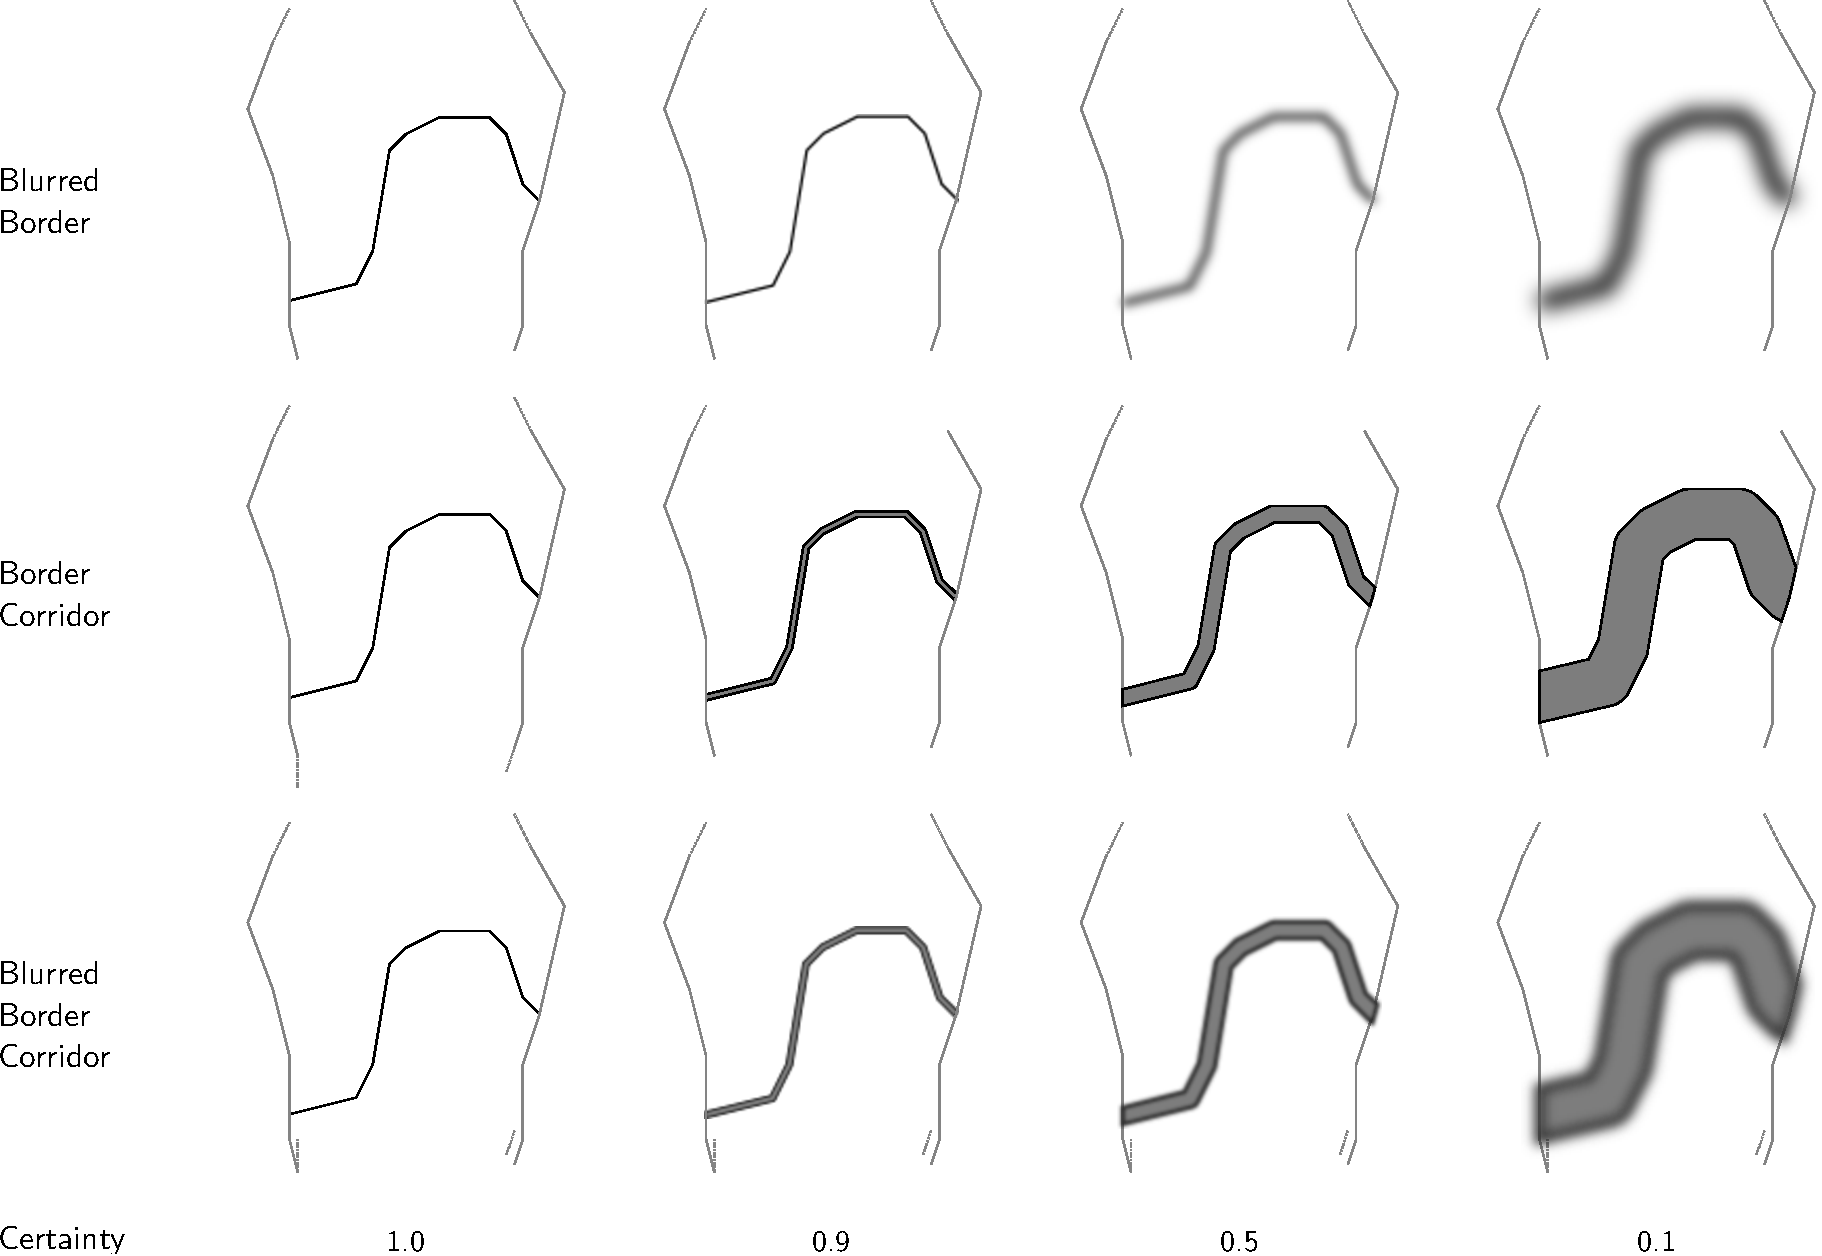
\includegraphics[width = 0.8\textwidth]{graphics/5-uncertainty/border}
  \caption{Three different methods to visualize uncertain courses of a border}
  \label{fig:uncertainty_border}
\end{figure}

Another advantage of the input of borderlines instead of territories is that once the model is further advanced, coastlines can be continuously changed according to an appropriate change model (see problem \ref{problem_general_coastlines}). This can be applied solely to the coastlines without affecting the interior borders.

A new border point automatically snaps to an existing border point, if the mouse position is close enough to it (an appropriate threshold might be $5~px$). This allows for a smooth workflow and is required to create closed polygons. In case the borderline is closed, it gets treated as a complete polygon and territory. When the user finished a territory by defining all surrounding polylines that create a closed ring, the polygon gets assembled and the territory receives a background color. If a borderline meets another borderline at an interior node, the polyline gets split up into two parts so that each meeting point of borders is the start or end point of a polyline. This way integrity is maintained and each territory compounds of several polylines creating a set of closed polylines, a polypolygon.

\begin{figure}[ht]
  \centering
  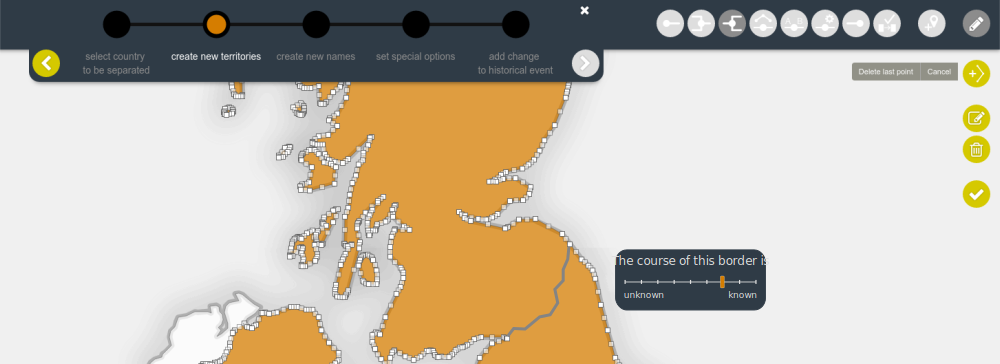
\includegraphics[width = 0.8\textwidth]{graphics/5-uncertainty/new_territory_tool}
  \caption{Drawing historical borders instead of full areas and definining a level of certainty.}
  \label{fig:uncertainty_new_territory_tool}
\end{figure}


(X) overlapping territories will create new areas that has to be tredted separately:
  contested area? part of other area?
(X) empty territories will create new areas that has to be tredted separately:
  unclaimed empty land? neutral zone?


\begin{figure}[ht]
  \centering
  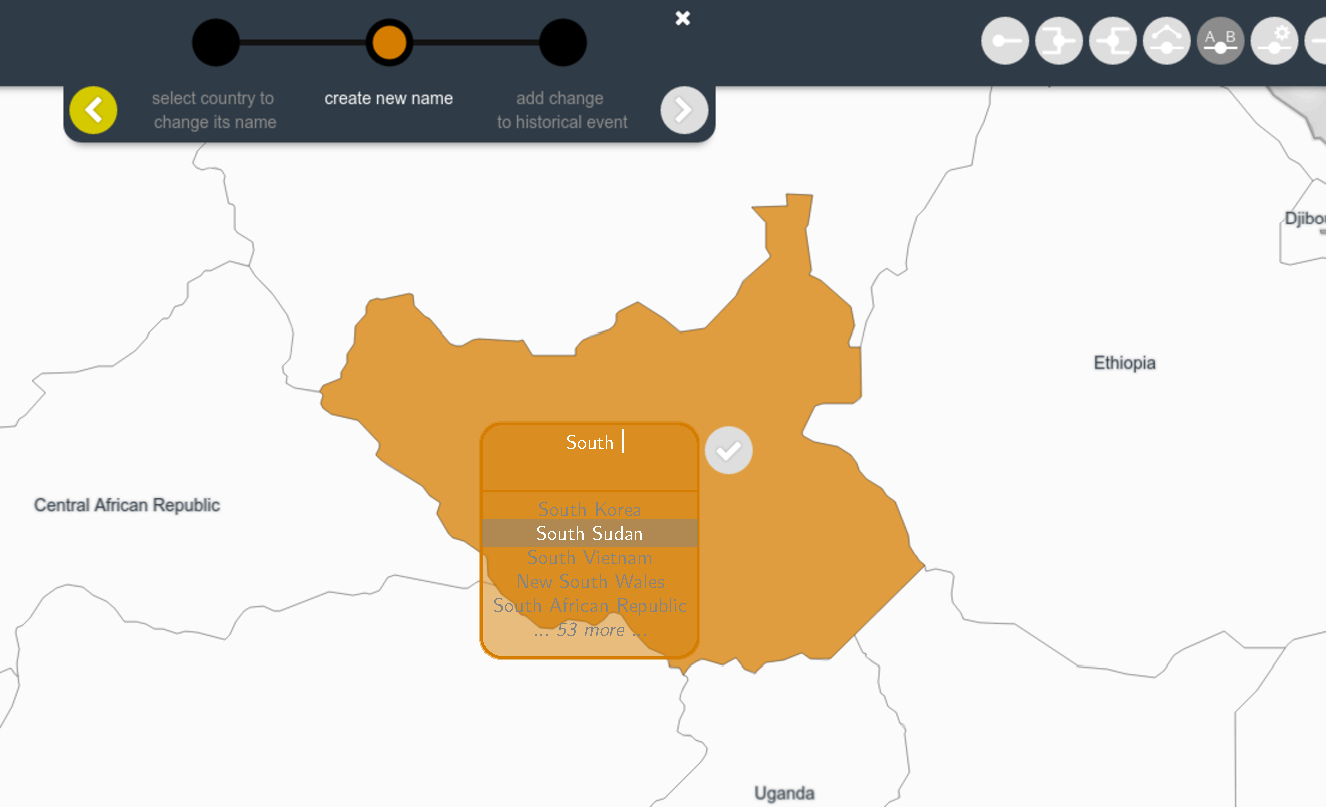
\includegraphics[width = 0.8\textwidth]{graphics/5-uncertainty/new_name_tool}
  \caption{Getting suggestions for the name name from Wikipedia.}
  \label{fig:uncertainty_new_name_tool}
\end{figure}


To treat special areas differently, a new step in the edit operation workflow gets defined: \textbf{Set New Status}

\begin{figure}[ht]
  \centering
  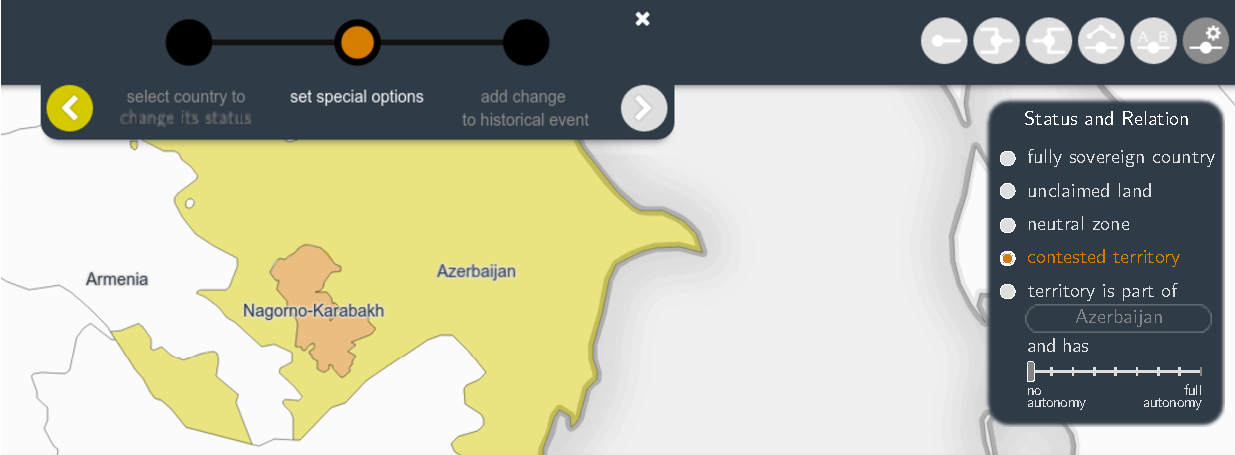
\includegraphics[width = 0.8\textwidth]{graphics/5-uncertainty/new_status_tool}
  \caption{Defining a special status or relationship to a territory.}
  \label{fig:uncertainty_new_status_tool}
\end{figure}


\begin{figure}[ht]
  \centering
  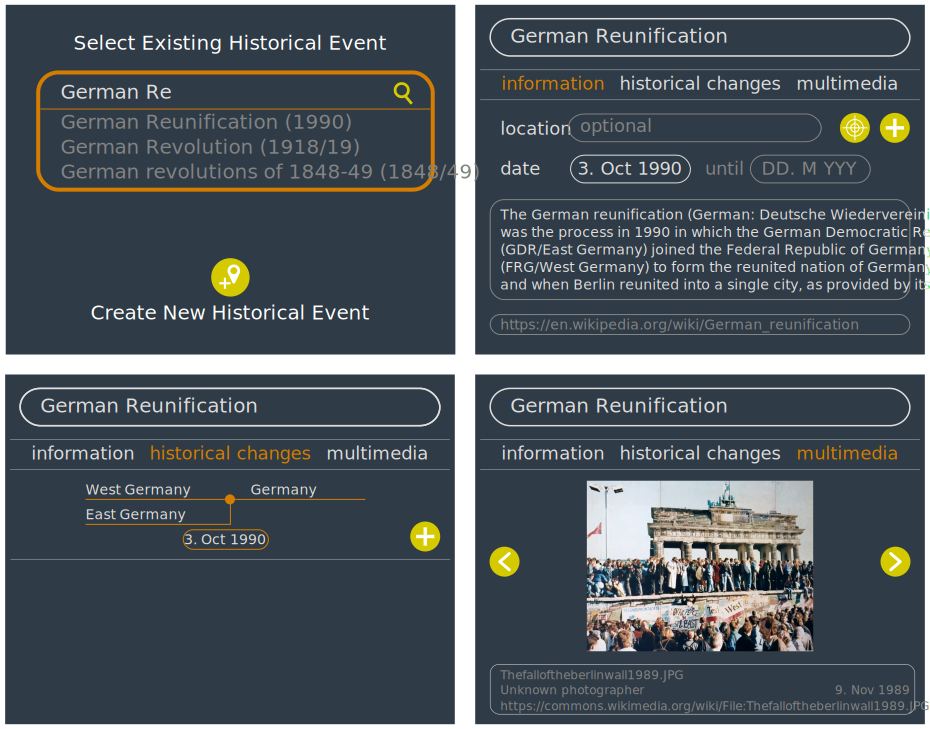
\includegraphics[width = 0.8\textwidth]{graphics/5-uncertainty/new_hivent_box}
  \caption{Creating a new Hivent and adding the newly created historical change.}
  \label{fig:uncertainty_new_hivent_box}
\end{figure}


\begin{figure}[ht]
  \centering
  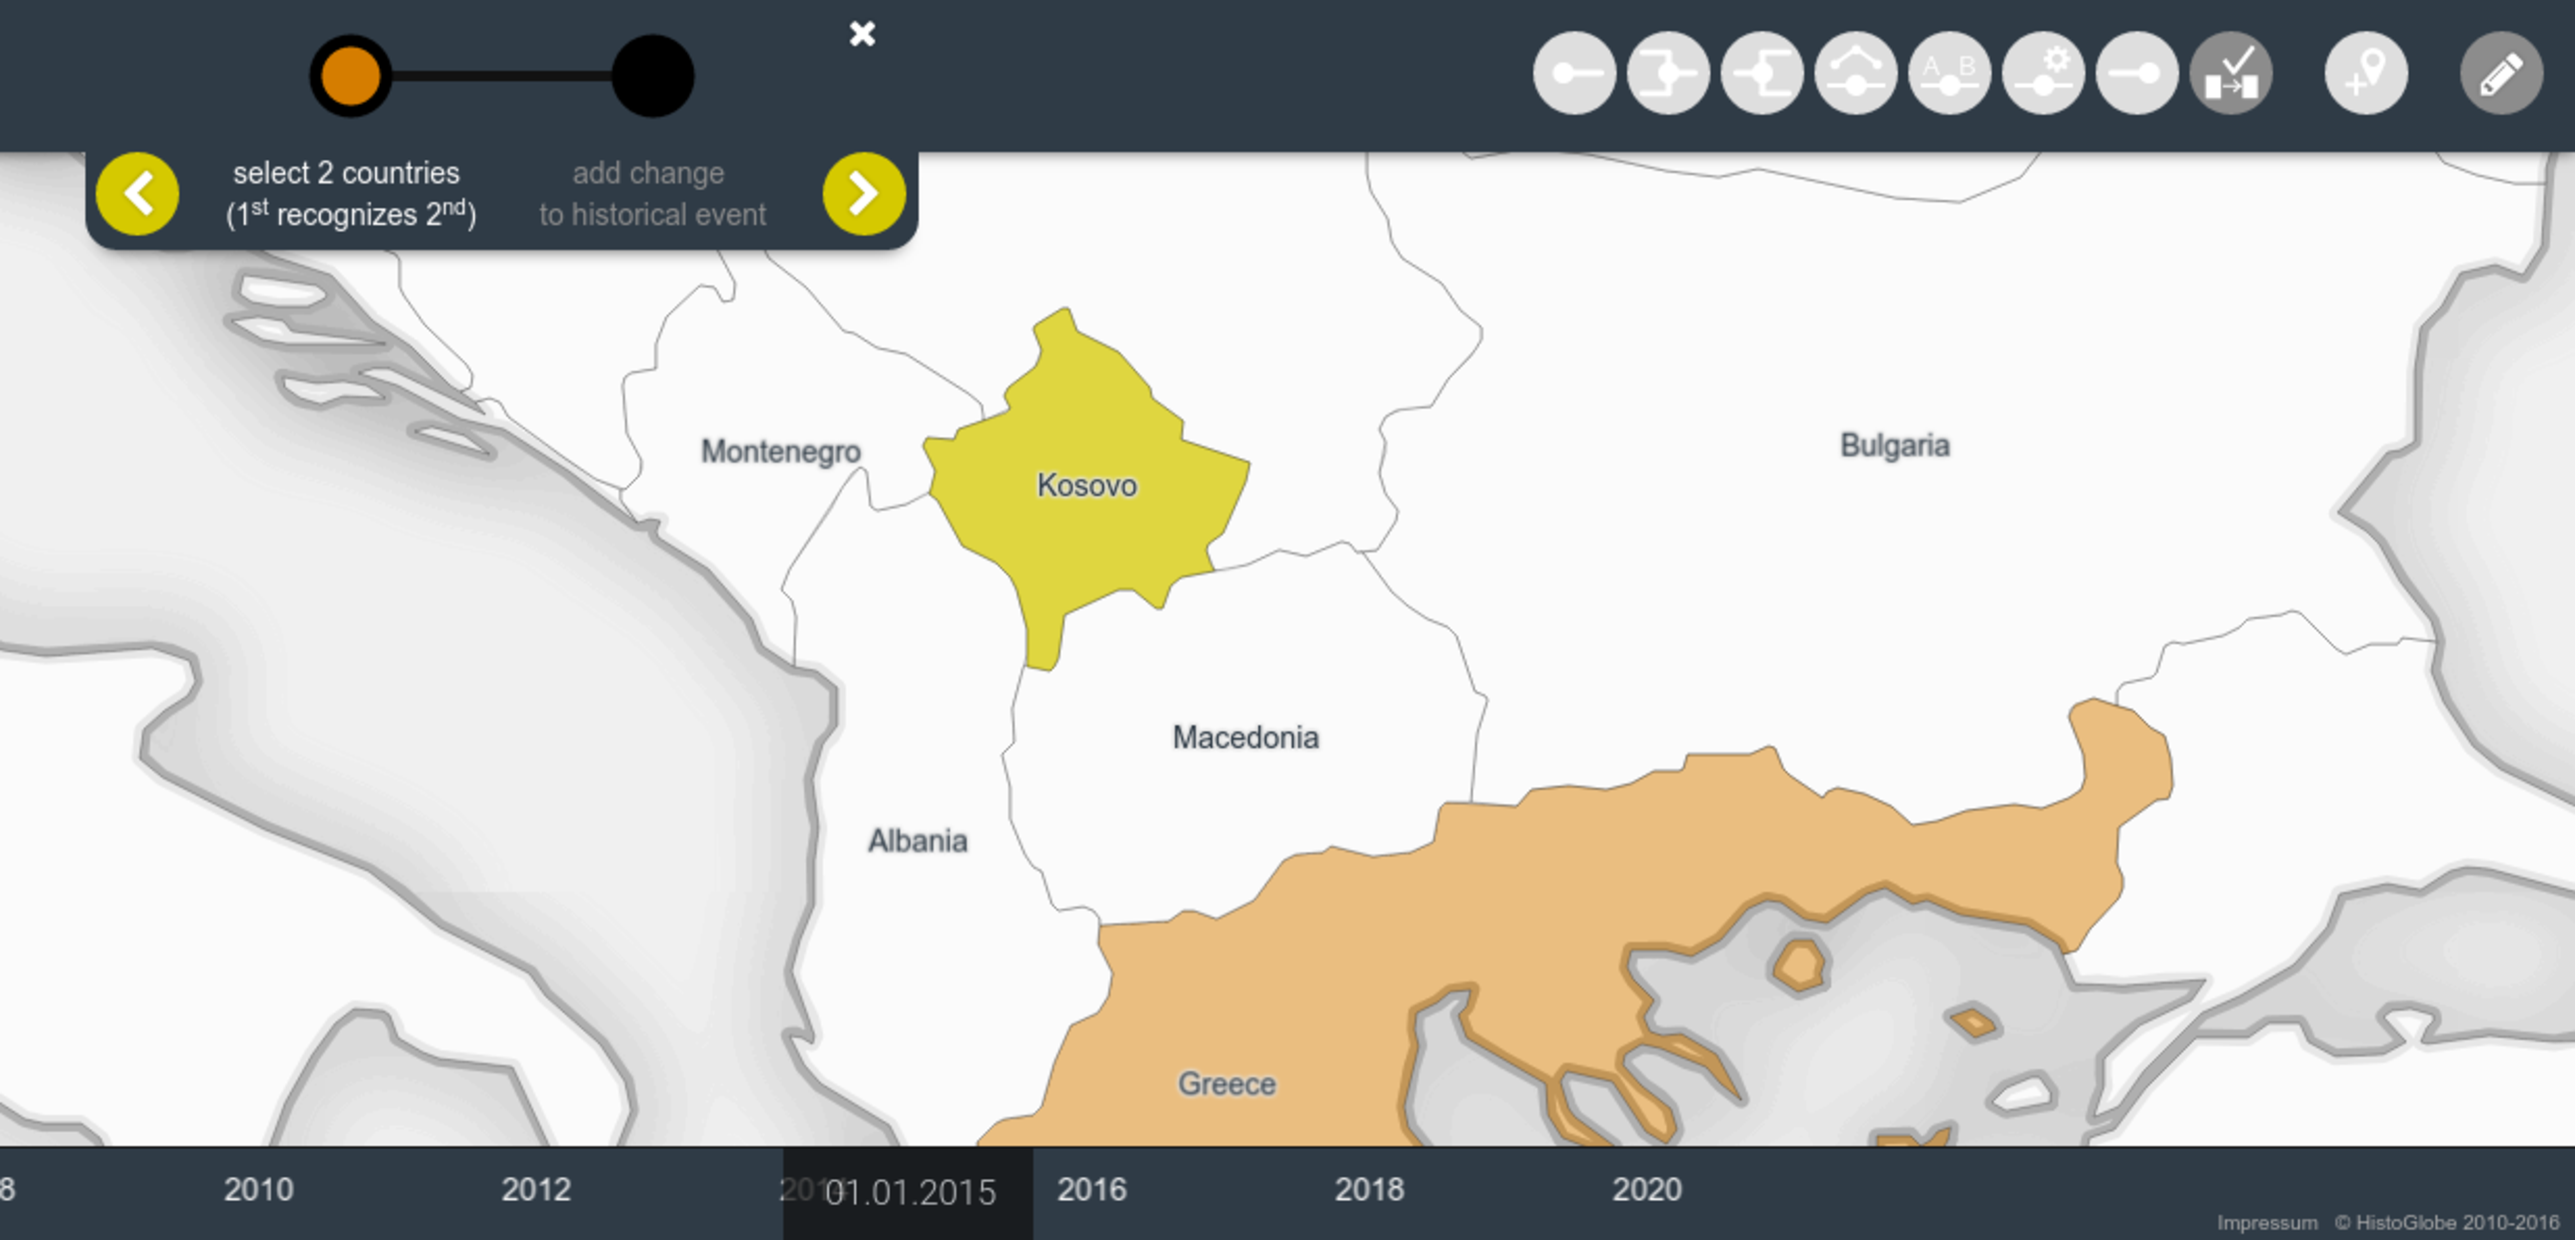
\includegraphics[width = 0.8\textwidth]{graphics/5-uncertainty/operation_REC}
  \caption{New edit operation: Recognition -- sets up the recognition of one area to another.}
  \label{fig:uncertainty_operation_REC}
\end{figure}

\newpage

SET\_NAME step:
(X) lookup name in Wikipedia collection of historical and current countries

new SET\_STAT step:
(X) set relation to other area by clicking on it, setting it as super-/subordinate and assigning autonomy level:
no autonomy |----*| fully sovereign
(X) set status of area in dialogue (unclaimed, contested, neutral, part of => correction)


ADD\_CHNG step:
(-) find Hivent name in Wikipedia articles


In order to support different languages, a language selection is placed on the bottom right corner of the interface, on the timeline (see figure \ref{fig:multi_language}). This changes the language of the whole interface and loads the translations of the historical events, locations and area names in the newly created language. If a term is not defined in the language, the fallback language (English) is used instead.
\begin{figure}[ht]
  \centering
  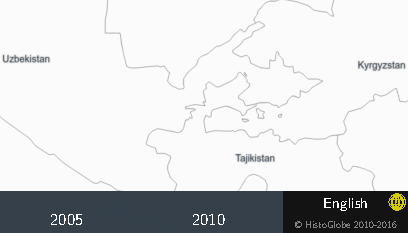
\includegraphics[width = 0.45\textwidth]{graphics/5-uncertainty/multi_language}
  \caption{Changing the language in the user interface.}
  \label{fig:multi_language}
\end{figure}




% subsubsection extension_of_the_edit_mode (end)

% ------------------------------------------------------------------------------
\subsubsection{Extension of the data model} % (fold)
\label{ssub:extension_of_the_data_model}


\begin{figure}[ht]
  \centering
  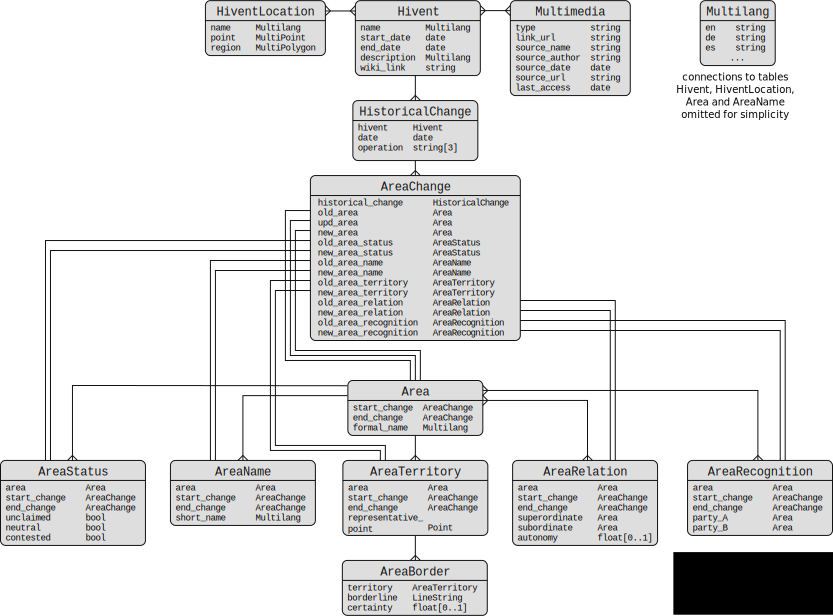
\includegraphics[width = 0.8\textwidth]{graphics/5-uncertainty/new_data_model}
  \caption{The extended data model to support various kinds of uncertainty and disagreement}
  \label{fig:new_data_model}
\end{figure}


Wikipedia synch
signing parties to account for bias toward the winner
multiple locations
-> for each location: geocoding (location name -> point / region)
multiple dates, multiple effect dates <-> HistoricalChange
two views:
* Hivent name + metadata
* Hivent name + description + multimedia


formal name = identity => move to Area
new entity: AreaRelation    (superordinate, subordinate, autonomy € [0..1[ )
new entity: AreaRecognition (party\_A, party\_B)
new entity: AreaStatus      (neutral, contested)

disagreement can be handled by modelling overlapping territories, that more than one entity claims, separately

% subsubsection extension_of_the_data_model (end)

% subsection solution_approaches (end)


% ==============================================================================

% section uncertainty (end)